\documentclass{article}

% to compile a preprint version, e.g., for submission to arXiv, add add the
% [preprint] option:
\usepackage[preprint]{neurips_2020}
\usepackage{hyperref}       % hyperlinks
\usepackage{url}            % simple URL typesetting
\usepackage{caption}
\usepackage{graphicx}

\linespread{1.25}

\title{DpicNet: A Transfer Learning Approach Towards Intel Multiclass Image Classification Dataset}

\author{%
  Xiaotong Niu \\
  Boston University\\
  \texttt{silnuext@bu.edu} \\
  \And
  Phumin Walaipatchara \\
  Boston University\\
  \texttt{phuminw@bu.edu} \\
}

\begin{document}

\maketitle

\begin{abstract}
  This paper talks about DpicNet, a transfer learning approach taken towards the Intel Multi-class Image Classification Challenge. DpicNet, roughly speaking, is a convolutional neural network that combines transfer learning with Xception architecture for the purpose of predicting images into different categories of natural scenes. After series of experiments with various structures, DpicNet shows its great results overall in both training and testing dataset in their loss and accuracy performances, and it successfully predicts most of the images correctly in the designated prediction set of images.
\end{abstract}

% ==========================================================================

\section{Introduction and Background}

As the technique of machine learning and deep learning emerges and boosts in the past few years, using them on image processing has become a popular topic in the field. More works have been done regarding using images to do predictions and recognitions on specific topics. In the year of 2018, Intel hosted a Image/Scene Classification Challenge as an encouragement for the public to get familiar with their novel OpenVINO toolkit - a tool that was designed by Intel for machine learning uses regarding image processing. The challenge itself asked the participants to build a deep learning model that recognize types of items contained in certain images into 6 main categories: buildings, forest, glacier, mountain, sea, and street. DpicNet strictly follows the purpose of the challenge and was designed to become a system that uses its own, novel approach to do the classification, using technologies of combining the transfer learning method with Xception model, a model that act as an improvement for the famous Inception V3 model.

\subsection{Dataset}

The dataset DpicNet targeted is located at \href{https://www.kaggle.com/puneet6060/intel-image-classification}{Intel Multi-class Image Classification} which was originally published by Intel  containing images of natural scenes around the world. There are a total of 25,000 images within 6 categories that are categorized to be classified: buildings, forest, glacier, mountain, sea, and street, each with a size of 150 x 150 pixels. The images are split into roughly 14,000 images for training, 3,000 images for testing, and 7,000 images for prediction. All of the Images are preprocessed to match the input requirement of the Xception model.

% ==========================================================================

\section{Prior Works}

Being a challenge hosted by a well-known company, this challenge had various number of submission across the internet and continues to receive new presentations from data scientists on Kaggle. Thus, we researched through several previous works before we could actually start designing DpicNet. There are two of them that helped us get a general idea on how things work around in this project mostly. One was an approach uses basic CNN posted by Vince. This approach uses Conv2D in the first few layers and DenseNet in the last few layers, with the combination of using ReLU activation function and softmax activation function in its last layer, achieved overall a decent result of 83\% on the testing dataset. Another work we found helpful was a series of approaches published by Sai Nikhilesh. He proposed a total of 5 approaches, including Conv2d which achieves about 80\% in accuracy, VGG19 which uses softmax activation function and achieves about 86\% in accuracy, EfficientNetB7 which uses Adam activation function and DenseNet121 which uses RMSprop activation function and categorical\_smooth\_loss loss function but both did not achieve good results, and his best approach DenseNet201 which achieves about 90\% of accuracy.

% ==========================================================================

\section {Methodology}

The basic implementation idea of DpicNet is to use transfer learning from Xception model, plus the usage of Keras and Tensorflow in training our data and Boston University Shared Computing Cluster in testing our data. We first transfer the convolutional parts of Xception and freeze it, then conducted experiments on various fully-connected network structures from Xception. For the output nodes, we use softmax function as our activation function and we use categorical cross-entropy function as our loss function.

Our settings on variants includes changing number of nodes in hidden layers, adding more hidden layers, and imposing regularization to the hidden layers. In all variant settings that we determined, all hidden layers are incorporated with a bias term.

\subsection{Transfer Learning}

Transfer learning is an approach of customizing networks that have been trained to a designated dataset, which here is ImageNet. By using transfer learning in DpicNet, we don't have to put too much effort on how exactly to train the data but rather have a dataset that has been trained and a way of training it, then extend everything to our own training dataset. 

\subsection{Xception}

Xception is much more alike Inception V3 as mentioned in earlier paragraphs. Basically, it is an architecture that has the same number of parameters as in Inception V3 but only with a smaller model size. What makes it exceptional is that the overall performance for Xception slightly outperforms Inception V3. While the performance gains are not due to the increased capacity, it gains from a more efficient use of the model parameters. Plus, the fact that it has already been trained on ImageNet dataset saved us a great amount of effort in researching.

% ==========================================================================

\section{Results}

We grouped our network structures into 3 categories: no regularization, with regularization, and more hidden layers. We are aiming to examine how each factor affects the network performance and will figure out the most optimal setting among all structures experimented.
\\
Regarding regularization experiment, we chose Structure 4 as a base structure and the regularization techniques to be experimented are L1 and L2. We tested applying L1 regularization to both hidden layers; however, the network exhibits very poor performance with less than 20\% accuracy. Therefore, this setting is not included. We also tested applying L1 regularization to one layer and L2 regularization to another layer, but this setting exhibits mediocre performance with about 67\% accuracy. Therefore, this setting is not included as well.
\\
Adding more hidden layers increases the model parameters while enables more capability to fit the data better. We are going to experiment whether adding more layers (from 2 to 3) can decrease the loss and increase the accuracy on the data (training, testing, predict). Moreover, we are going to examine the tradeoff between growth in parameters, which requires more training time and consumes more space, and accuracy on the data.
\\
The experiment result is shown in Table \ref{t2:acc_loss_train_tab} and Table \ref{t3:acc_loss_test_tab} where most structures perform well on training data except Structure 6. In spite of that, Structure 6 performs well on testing dataset as well as Structure 3 that exhibits good performance on testing data with low loss and highest accuracy. Structure 3 seems to be the best among all structures experimented considering the metrics (loss, accuracy) and the number of parameters in the network.

\begin{table}[h]
    \centering
    \begin{tabular}{|c|c|c|c|c|}
        \hline
         \#&Hidden Layers&Hidden Nodes&Bias&Regularization\\
         \hline
         1&2&512,128&Yes&No\\
         \hline
         2&2&2048,1024&Yes&No\\
         \hline
         3&2&256,32&Yes&No\\
         \hline
         4&2&8192,1024&Yes&No\\
         \hline
         5&2&16384,4096&Yes&No\\
         \hline
         6&2&8192,1024&Yes&L2,L2\\
         \hline
         7&3&8192,1024,256&Yes&No\\
         \hline
         8&3&8192,1024,512&Yes&No\\
         \hline
    \end{tabular}
    \caption{Network Structures}
    \label{t1:net_struct}
\end{table}

% \subsection{No Regularization}
% We started by constructing the hidden layers of the fully-connected part without any regularization
% \subsubsection{Structure 1}

% In this structure, we designed the top parts of DpicNet to have 2 hidden layers with 512 and 128 nodes, respectively. All hidden layers are incorporated with a bias term, but no regulatization is applied to either the weight or the bias term.

% \subsubsection{Structure 2}

% In this structure, we increased the number of nodes of 2 hidden layers from Structure 1 to be 2048 and 1024 nodes, respectively. All hidden layers are incorporated with a bias term, but no regularization is applied to either the weight or the bias term.

% \subsubsection{Structure 3}

% In this structure, we decreased the number of nodes of 2 hidden layers from Structure 1 to be 256 and 32 nodes, respectively. All hidden layers are incorporated with a bias term, but no regularization is applied to either the weight or the bias term.

% \subsubsection{Structure 4}

% In this structure, we increased the number of nodes of 2 hidden layers from Structure 1 to be 8192 and 1024 nodes, respectively. All hidden layers are incorporated with a bias term, but no regularization is applied to either the weight or the bias term.

% \subsubsection{Structure 5}

% In this structure, we increased the number of nodes of 2 hidden layers from Structure 1 to be 16384 and 4096 nodes, respectively. All hidden layers are incorporated with a bias term, but no regularization is applied to either the weight or the bias term.

% \subsection{With Regularization}

% We are going to add different types of regularization to our network and examine the difference in performance. We choose Structure 4 as a base structure and the regularization techniques to be experimented are L1, L2, and L1 and L2. We tested applying L1 regularization to both hidden layers; however, the network exhibits very poor performance with less than 20\% accuracy. Therefore, this setting is not included in this section. We also tested applying L1 regularization to one layer and L2 regularization to another layer, but this setting exhibits mediocre performance with about 67\% accuracy. Therefore, this setting is not included in this section as well.

% \subsubsection{Structure 6}

% In this structure, there are two hidden layers with 8192 and 1024 nodes, same as Structure 4, and those layers are incorporated with a bias term. In addition, L2 regularization is applied to both layers

% \subsection{Three hidden layers with no Regularization}

% Adding more hidden layers increases the model parameters while enables more capability to fit the data better. We are going to experiment whether adding more layers (from 2 to 3) can decrease the loss and increase the accuracy on the data (training, testing, predict). Moreover, we are going to examine the tradeoff between growth in parameters, which requires more training time and consumes more space, and accuracy on the data.

% \subsubsection{Structure 7}

% Based on Structure 4, this structure differs by adding one more hidden layer on top of the existing hidden layers in Structure 4 with 256 nodes. All hidden layers are incorporated with a bias term and no regularization of any kind is applied to any hidden layer.

% \subsubsection{Structure 8}

% This structure is almost identical with Structure 7, except that the number of nodes in the newly added hidden layer is changed to 512.

% ==========================================================================

\section{Performance Discussion}

We recorded the loss and accuracy of each structure on training and testing dataset. Loss function used is categorical cross-entropy loss function. The batch size for all experiments is 32. 

\subsection{Training Data}
Because of batch size of 32, each epoch contains 439 steps. The experiment result of each structure is shown in Table 1. From the experiment result, Structure 2, 4, and 7 are outstanding in terms of accuracy at epoch 10. Structure 6, which incorporated L2 regularization to both layers, does not exhibit impressive performance despite training up to 40 epochs. Structure 7 and 8, which have 3 hidden layers with different number of nodes in the last hidden layer, performs well compared to Structure 1 - 4; however, adding more hidden layer does not significantly improve the performance on the training dataset.

\begin{table}[]
  \centering
  \begin{minipage}[b]{0.23\linewidth}
  \tiny
  \begin{tabular}{|c|c|c|}
    \hline
    Epoch&Loss&Accuracy\\
    \hline
    1&0.7697&0.781\\
    \hline
    2&0.3522&0.8758\\
    \hline
    3&0.2424&0.9120\\
    \hline
    4&0.1798&0.9362\\
    \hline
    5&0.1248&0.9557\\
    \hline
    6&0.1135&0.9608\\
    \hline
    7&0.1253&0.9589\\
    \hline
    8&0.0786&0.9734\\
    \hline
    9&0.0696&0.9786\\
    \hline
    10&0.0713&0.9784\\
    \hline
  \end{tabular}
  \caption*{Structure 1}
  \end{minipage}
  \hspace{0.5cm}
  \begin{minipage}[b]{0.23\linewidth}
  \tiny
  \begin{tabular}{|c|c|c|}
    \hline
    Epoch&Loss&Accuracy\\
    \hline
    1&1.0170&0.7748\\
    \hline
    2&0.3853&0.8619\\
    \hline
    3&0.2634&0.9043\\
    \hline
    4&0.1818&0.9348\\
    \hline
    5&0.1483&0.9479\\
    \hline
    6&0.1179&0.9577\\
    \hline
    7&0.0871&0.9701\\
    \hline
    8&0.1059&0.9672\\
    \hline
    9&0.0648&0.9800\\
    \hline
    10&0.0526&0.9838\\
    \hline
  \end{tabular}
  \caption*{Structure 2}
  \end{minipage}
  \hspace{0.5cm}
  \begin{minipage}[b]{0.23\linewidth}
  \tiny
  \begin{tabular}{|c|c|c|}
    \hline
    Epoch&Loss&Accuracy\\
    \hline
    1&0.7723&0.7590\\
    \hline
    2&0.3895&0.8669\\
    \hline
    3&0.2822&0.9015\\
    \hline
    4&0.2205&0.9220\\
    \hline
    5&0.1826&0.9384\\
    \hline
    6&0.1295&0.9555\\
    \hline
    7&0.1031&0.9648\\
    \hline
    8&0.1051&0.9656\\
    \hline
    9&0.0784&0.9730\\
    \hline
    10&0.0912&0.9705\\
    \hline
  \end{tabular}
  \caption*{Structure 3}
  \end{minipage}
  \\
  \begin{minipage}[b]{0.23\linewidth}
  \tiny
  \begin{tabular}{|c|c|c|}
    \hline
    Epoch&Loss&Accuracy\\
    \hline
    1&1.7312&0.7761\\
    \hline
    2&0.3870&0.8603\\
    \hline
    3&0.2559&0.9063\\
    \hline
    4&0.1886&0.9333\\
    \hline
    5&0.1396&0.9513\\
    \hline
    6&0.1151&0.9618\\
    \hline
    7&0.0848&0.9726\\
    \hline
    8&0.0832&0.9734\\
    \hline
    9&0.0846&0.9748\\
    \hline
    10&0.0515&0.9840\\
    \hline
  \end{tabular}
  \caption*{Structure 4}
  \end{minipage}
  \hspace{0.5cm}
  \begin{minipage}[b]{0.23\linewidth}
  \tiny
  \begin{tabular}{|c|c|c|}
    \hline
    Epoch&Loss&Accuracy\\
    \hline
    1&2.4641&0.7775\\
    \hline
    2&0.3616&0.8706\\
    \hline
    3&0.2905&0.9042\\
    \hline
    4&0.2051&0.9287\\
    \hline
    5&0.1535&0.9471\\
    \hline
    6&0.1257&0.9583\\
    \hline
    7&0.1538&0.9603\\
    \hline
    8&0.0834&0.9722\\
    \hline
    9&0.0683&0.9776\\
    \hline
    10&0.0730&0.9797\\
    \hline
  \end{tabular}
  \caption*{Structure 5}
  \end{minipage}
  \hspace{0.5cm}
  \begin{minipage}[b]{0.23\linewidth}
  \tiny
  \begin{tabular}{|c|c|c|}
    \hline
    Epoch&Loss&Accuracy\\
    \hline
    1&11.6508&0.7146\\
    \hline
    2&2.7279&0.7545\\
    \hline
    3&2.0377&0.7770\\
    \hline
    4&2.0157&0.7779\\
    \hline
    5&1.7358&0.7926\\
    \hline
    6&1.5305&0.8003\\
    \hline
    7&1.3250&0.8088\\
    \hline
    8&1.2319&0.8123\\
    \hline
    9&1.1533&0.8154\\
    \hline
    10&1.0536&0.8180\\
    \hline
    20&0.7546&0.8336\\
    \hline
    30&0.6780&0.8423\\
    \hline
    40&0.6588&0.8439\\
    \hline
  \end{tabular}
  \caption*{Structure 6}
  \end{minipage}
  \\
  \begin{minipage}[b]{0.23\linewidth}
  \tiny
  \begin{tabular}{|c|c|c|}
    \hline
    Epoch&Loss&Accuracy\\
    \hline
    1&1.4817&0.7720\\
    \hline
    2&0.3707&0.8663\\
    \hline
    3&0.2519&0.9057\\
    \hline
    4&0.1884&0.9317\\
    \hline
    5&0.1469&0.9512\\
    \hline
    6&0.1170&0.9632\\
    \hline
    7&0.0929&0.9694\\
    \hline
    8&0.0954&0.9708\\
    \hline
    9&0.0886&0.9721\\
    \hline
    10&0.0597&0.9818\\
    \hline
  \end{tabular}
  \caption*{Structure 7}
  \end{minipage}
  \hspace{0.5cm}
  \begin{minipage}[b]{0.23\linewidth}
  \tiny
  \begin{tabular}{|c|c|c|}
    \hline
    Epoch&Loss&Accuracy\\
    \hline
    1&1.3941&0.7753\\
    \hline
    2&0.3921&0.8603\\
    \hline
    3&0.2674&0.9026\\
    \hline
    4&0.1950&0.9303\\
    \hline
    5&0.1589&0.9466\\
    \hline
    6&0.1189&0.9608\\
    \hline
    7&0.0974&0.9676\\
    \hline
    8&0.0669&0.9778\\
    \hline
    9&0.0771&0.9766\\
    \hline
    10&0.0724&0.9780\\
    \hline
  \end{tabular}
  \caption*{Structure 8}
  \end{minipage}
  \caption{Accuracy and Loss on Training Data}
  \label{t2:acc_loss_train_tab}
\end{table}

\subsection{Testing Data}

After training, each structure was tested on testing data using batch size of 32 and the testing was done after 94 steps. The performance is evaluated based on accuracy on the testing data and shown in Table 2. Structure 3 performs the best among all structures experimented despite no regularization applied and less hidden layers.

\begin{table}[h]
    \centering
    \begin{tabular}{|c|c|c|}
    \hline
    \#&Loss&Accuracy\\
    \hline
    1&1.142&0.828\\
    \hline
    2&1.573&0.808\\
    \hline
    3&0.843&0.867\\
    \hline
    4&1.384&0.843\\
    \hline
    5&1.730&0.838\\
    \hline
    6&0.706&0.824\\
    \hline
    7&1.646&0.788\\
    \hline
    8&1.689&0.837\\
    \hline
    \end{tabular}
    \caption{Accuracy and Loss on Testing Data}
    \label{t3:acc_loss_test_tab}
\end{table}

\subsection{Prediction Data}

We chose Structure 6, which performs the best on testing data in terms of loss, instead of other good performers on training data since the model can perform impressively on training data by fitting into the training data, but might not be able to generalize to unseen data like testing data.

\begin{center}
    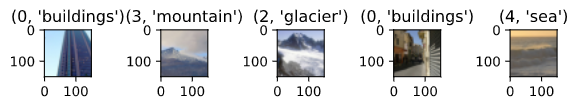
\includegraphics[scale=0.68]{assets/s6.png}
\end{center}

Five random images are chosen from images under \textit{src/data/predict/} directory. These images do not have label, so we are going to evaluate based on our knowledge whether the prediction is acceptable. The result is quite impressive as all five images are classified into their correct categories despite abut 82\% accuracy on testing data.

% ==========================================================================

\section{Conclusion and Future Works}

Taking look back at DpicNet, this model does a fairly good job in both the performance analysis consideration and the prediction result consideration. The overall performance in both loss and accuracy is acceptable and in a good standard regarding different number of nodes, layers, epochs, with and without regularization. Thus overall, it completes the challenge and achieves the desired result.

As for future improvements regarding what is in the current DpicNet, we do believe that regularization plays some role in our performance. Yet we would still need further experimental steps to analyze whether it actually hurts or boosts the performance. Furthermore, after more tests on the current DpicNet has done, we would probably consider exploiting other ways of implementations beside fully-connected network and see if the accuracy could be improved to over 90\% so that our prediction result could be in more precision.

% ==========================================================================

\begin{thebibliography}{9}
% reference
    \bibitem{xceptionpaper1}
    François Chollet
    \textit{Xception: Deep Learning with Depthwise Separable Convolutions}.
    arXiv:1610.02357 cs.CV (2016)
    
    \bibitem{basiccnnkaggle}
    Vince
    \textit{Intel Image Classification (CNN - Keras)}.
    Kaggle (2020)
    
    \bibitem{5approachkaggle}
    Sai Nikhilesh
    \textit{Transfer learning beginner friendly code - 90\% acc}.
    Kaggle (2020)
    
    \bibitem{translearnCV}
    Jason Brownlee
    \textit{Transfer Learning in Keras with Computer Vision Models}.
    Machine Learning Mastery (2019)
\end{thebibliography}
\end{document}
